\begin{figure}[H]
    \centering
    \caption{Enumeration of self-avoiding paths in $\Z^2$}
    \label{fig:nb_self_avoiding_path}
    \minipage{0.5\textwidth}
    \centering
    \begin{tikzpicture}
        \foreach \i in {-1, 0, 1} {
            \draw[gray] (-1.5, \i) -- (1.5, \i);
            \draw[gray] (\i, -1.5) -- (\i, 1.5);
            \draw[gray, dashed] (-1.5, \i) -- (-2.0, \i);
            \draw[gray, dashed] (\i, -1.5) -- (\i, -2.0);
            \draw[gray, dashed] (1.5, \i) -- (2.0, \i);
            \draw[gray, dashed] (\i, 1.5) -- (\i, 2.0);
        }
        
        \filldraw (0, 0) circle (1pt);
        \draw[->, thick] (0, 0) -- (1, 0);
        \draw[->, thick] (0, 0) -- (0, 1);
        \draw[->, thick] (0, 0) -- (-1, 0);
        \draw[->, thick] (0, 0) -- (0, -1);
    \end{tikzpicture}
    \caption*{$4$ choices for the first step}
    \endminipage\hfill
    % --
    \minipage{0.5\textwidth}
    \centering
    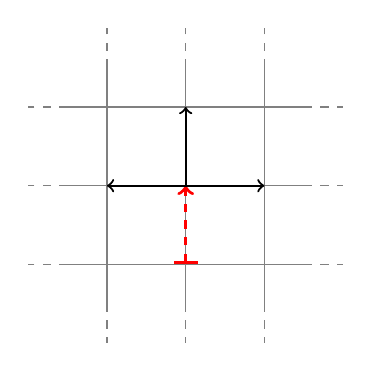
\begin{tikzpicture}
        \foreach \i in {-1, 0, 1} {
            \draw[gray] (-1.5, \i) -- (1.5, \i);
            \draw[gray] (\i, -1.5) -- (\i, 1.5);
            
            \draw[gray, dashed] (-1.5, \i) -- (-2.0, \i);
            \draw[gray, dashed] (\i, -1.5) -- (\i, -2.0);
            \draw[gray, dashed] (1.5, \i) -- (2.0, \i);
            \draw[gray, dashed] (\i, 1.5) -- (\i, 2.0);
        }
        
        \draw[|->, red, dashed, very thick] (0, -1) -- (0, 0);
        \draw[->, thick] (0, 0) -- (1, 0);
        \draw[->, thick] (0, 0) -- (0, 1);
        \draw[->, thick] (0, 0) -- (-1, 0);
    \end{tikzpicture}
    \caption*{$3$ choices for any step that follows}
    \endminipage
\end{figure}